 \documentclass[11pt, a4papper]{report}
\usepackage{amsthm}
\usepackage{amssymb, amsmath}
\usepackage{array}
%\usepackage[romanian]{babel}
\usepackage{bm}
%\usepackage{enumerate}
\usepackage{float}
\usepackage{geometry}
\usepackage{graphicx}
\usepackage{listings}
\usepackage{longtable}
%\usepackage{index}
\usepackage{minted}
%\usepackage{tikz}
%\usepackage{ucs}
\usepackage[utf8]{inputenc}

\theoremstyle{plain}
\newtheorem{theorem}{Theorem}

\theoremstyle{definition}
\newtheorem{definition}{Definition}

\theoremstyle{definition}
\newtheorem{lemma}{Lemma}

\theoremstyle{proposition}
\newtheorem{proposition}{Proposition}

 \geometry{
 a4paper,
 total={160mm,257mm},
 left=30mm,
 right=20mm,
 top=20mm,
 bottom=20mm,
 }
 
\setcounter{tocdepth}{4}
\setcounter{secnumdepth}{4}
\renewcommand{\baselinestretch}{1.25}
 
\graphicspath{ {Imagini/} }

\begin{document}

\begin{titlepage}

\begin{center}
\begin{large}
Universitatea ``Alexandru Ioan Cuza" din Iaşi\\
Facultatea de Informatică\\
\end{large}
\end{center}

\vspace{50mm}

\begin{center}

\includegraphics{fii.png}
\end{center}
 
\vspace{15mm}

\begin{center}
\begin{Large}
LUCRARE DE DISERTAŢIE
\end{Large}
\\
\
\\
\
\

\begin{Huge}
\textbf{A Model for Heart Sounds Segmentation and
Classification using Neural Networks}
\end{Huge}

\

propusă de

\end{center}

\vspace{30mm}

\textbf{Student:} Oriana-Maria Oniciuc

\textbf{Coordonator ştiinţific:} Conf. Dr. Liviu Ciortuz
\\
\
\\
\


\vfill

\begin{center}
\textbf{Sesiunea:} iulie

2018
\end{center}

\end{titlepage}
\newpage

\begin{titlepage}

\begin{center}
Universitatea ``Alexandru Ioan Cuza" din Iaşi\\
Facultatea de Informatică\\
\end{center}

\vspace{85mm}
 
\begin{center}
\begin{Huge}
\textbf{A Model for Heart Sounds Segmentation and
Classification using Neural Networks}
\end{Huge}
\end{center}
 
\vspace{60mm}

\textbf{Student:} Oriana-Maria Oniciuc

\textbf{Coordonator ştiinţific:} Conf. Dr. Liviu Ciortuz

\vfill

\begin{center}
\textbf{Sesiunea:} iulie

2018
\end{center}

\end{titlepage}

\newpage

\pagenumbering{arabic}
\setcounter{page}{2}

\begin{flushright}
Avizat,\\
\^Indrum\u ator Lucrare de Diserta\c tie,\\
Conf. Dr. Ciortuz Liviu
\\

Data 28.06.2018 \hspace{0.4cm} Semn\u atura \rule{3.5cm}{0.4pt}
\end{flushright}
\

\begin{center}
\textbf{DECLARA\c TIA privind originalitatea con\c tinutului lucr\u arii de diserta\c tie}
\end{center}
\

Subsemnata ONICIUC ORIANA-MARIA, cu domiciliu \^in loc.RĂDĂUȚI, n\u ascută la data de 19.12.1994, identificat prin CNP 2941219226760, absolvent a Universit\u a\c tii ,,Alexandru Ioan Cuza" din Ia\c si, Facultatea de Informatic\u a, specializarea Informatic\u a, promo\c tia 2016-2018, declar pe propria r\u aspundere, cunosc\^and consecin\c tele falsului \^in declara\c tii \^in sensul art. 326 din Noul Cod Penal \c si dispozi\c tiile Legii Educa\c tiei Na\c tionale nr. 1/2011 art.143 al. 4 \c si 5 referitoare la plagiat, c\u a lucrarea de disertatie cu titlul: \textbf{\textit{A Model for Heart Sounds Segmentation and Classification using Neural Networks}}, elaborat\u a sub \^indrumarea dl. Conf. Dr. Ciortuz Liviu, pe care urmeaz\u a s\u a o sus\c tin \^in fa\c ta comisiei este original\u a, \^imi apar\c tine \c si \^imi asum con\c tinutul s\u au \^in \^intregime. De asemenea, declar c\u a sunt de acord ca lucrarea mea de disertație s\u a fie verificat\u a prin orice modalitate legal\u a pentru confirmarea originalit\u a\c tii, consim\c tind inclusiv la introducerea con\c tinutului s\u au \^intr-o baz\u a de date \^in acest scop. Am luat la cuno\c stin\c t\u a despre faptul c\u a este interzis\u a comercializarea de lucr\u ari \c stiin\c tifice \^in vederea facilit\u arii falsific\u arii de c\u atre cump\u ar\u ator a calit\u a\c tii de autor al unei lucr\u ari de licen\c t\u a, de diploma sau de diserta\c tie \c si \^in acest sens, declar pe proprie r\u aspundere c\u a lucrarea de fa\c t\u a nu a fost copiat\u a, ci reprezint\u a rodul cercet\u arii pe care am \^intreprins-o.

\bigskip
\

\noindent Data azi,

\noindent \rule{3.5cm}{0.4pt}
\


\begin{flushright}
  Oniciuc Oriana-Maria
  
  \rule{3.5cm}{0.4pt}
\end{flushright}

\newpage
\
\\
\


\begin{center}
DECLARA\c TIE DE CONSIM\c T\u AMÂNT
\end{center}

\bigskip

\indent
\par Prin prezenta declar c\u a sunt de acord ca Lucrarea de disertație cu titlul "A Model for Heart Sounds Segmentation and Classification using Neural Networks", codul surs\u a al programelor \c si celelalte con\c tinuturi (grafice, multimedia, date de test
etc.) care înso\c tesc aceast\u a lucrare s\u a fie utilizate în cadrul Facult\u a\c tii de Informatic\u a.
De asemenea, sunt de acord ca Facultatea de Informatic\u a de la Universitatea "Alexandru Ioan
Cuza" Ia\c si s\u a utilizeze, modifice, reproduc\u a \c si s\u a distribuie în scopuri necomerciale
programele-calculator, format executabil \c si surs\u a, realizate de mine în cadrul prezentei
lucr\u ari de disertație.
\\

\noindent Ia\c si,

\noindent 28.06.2018
\


\begin{flushright}
  Oniciuc Oriana-Maria
  
  \rule{3.5cm}{0.4pt}
\end{flushright}
\newpage

\vspace{10mm}
\begin{abstract}
\

This study aims is to produce a method that classifies phonocardiograms corresponding to different heart symptoms that are extremely subtle and challenging to separate. The problem is of particular interest to machine learning researchers as it involves classification of audio sample data, where distinguishing between classes of interest is non-trivial. Data is gathered in real-world situations and frequently contains background noise of every conceivable type.
\\

Some attempts to segment phonocardiograms (PCG) into heartbeats can be found in the literature. The characteristics of the PCG signal and other features such as heart sounds S1 and S2 location can be measured more accurately by digital signal processing techniques. We normalized the data using the $L^2$ norm and used a sliding window technique for which we used a peak detection algorithm. The models we used in classification are CNN and Adaboost.
\\

For the classification task some of the representative work that was done, has been presented in Classifying Heart Sounds Workshop. The teams used the J48 and MLP algorithms (using Weka) to train and classify the computed features, or exploit domain knowledge and compares the features of heartbeat before and after dropping out extra peaks and the smallest interval, used partial least squares regression, neural networks and convolution neural networks. The classification task in this project aims to give an alternative architecture for the model using Convolution Neural Network.
\end{abstract}

\newpage

%\pagenumbering{gobble}
%\

%\vspace{60mm}
%\
%
%\textbf{Mulţumiri}
%\\
%
%\
%
%Îmi doresc să mulţumesc celor care m-au susţinut în conceperea acestei lucrări. Sunt pe deplin recunoscătoare coordonatorului ştiinţific, conf. dr. Cristian Gaţu. Am învăţat foarte multe de la dumnealui şi m-a ghidat de fiecare dată spre rezultate foarte bune. Vreau să mulţumesc şi întregului corp profesoral care m-a îndrumat în aceşti ani nu doar ca excelenţi dascăli, ci mai ales ca modele pentru o carieră viitoare. De asemenea sunt recunoscătoare dragei mele familii şi tuturor colegilor extraordinari care mi-au fost alături în tot acest timp.
%
%\clearpage
%
%\newpage
\pagenumbering{arabic}
\setcounter{page}{5}
\addcontentsline{toc}{chapter}{Contents}

\tableofcontents

\newpage

\addcontentsline{toc}{chapter}{I. Introduction}
\chapter*{I. Introduction}

\

According to the World Health Organization, ischaemic heart disease and stroke are the world’s biggest killers, accounting for 15.2 million deaths in 2016. These diseases have remained the leading causes of death globally in the last 15 years. \cite{1} Any work done in detecting signs of heart disease could therefore have a significant impact on world health.
\\

Classifying Heart Sounds PASCAL provides us with a dataset that is gathered in real-world situations. Many recordings from the dataset contain background noise, being recorded both in a hospital environment by a doctor (using a digital stethoscope) and at home by the patient (using a mobile device). Success in classifying this form of data requires multiples preprocessing of the audio recordings. \cite{2} This dissertation presents an overview of two approaches to analysis and classification of heart sound signals. The main purpose of this study is developing an automatic methodology for identifying systole and diastole in the phonocardiograms and to classify the heartbeats in three classes.
\\

Big companies are interested in medical health activity which is one of the largest component of the economy. In 2017 Apple started to work with Stanford and American Well to determine if the heart rate sensor in the Apple Watch can be used to detect abnormal heart rhythms and common heart conditions. The study ended in 2018 and proved that the smart watch reaches a 97\% accuracy rate, 98\% sensitivity and 90\% specificity. \cite{3}


\addcontentsline{toc}{section}{I.1. Heart sounds}
\section*{I.1. Heart sounds}

\

The cardiac cycle is the performance of the human heart from the beginning of one heartbeat to the next one. In each cardiac cycle, the heart contracts (systole), pushing out the blood and pumping it through the body; this is followed by a relaxation phase (diastole), where the heart fills with blood, as illustrated in the next figure. 
\\

The atria contracts at the same time, forcing blood through valves into the ventricles. Closing of the atrioventricular valves produces a monosyllabic “lup” sound (S1). Following a brief delay, the ventricles contract at the same time forcing blood through the valves into the aorta and the artery transporting blood to the lungs. Closing of the semilunar valves produces a monosyllabic “dup” sound (S2). 
\\

\begin{figure}[h]
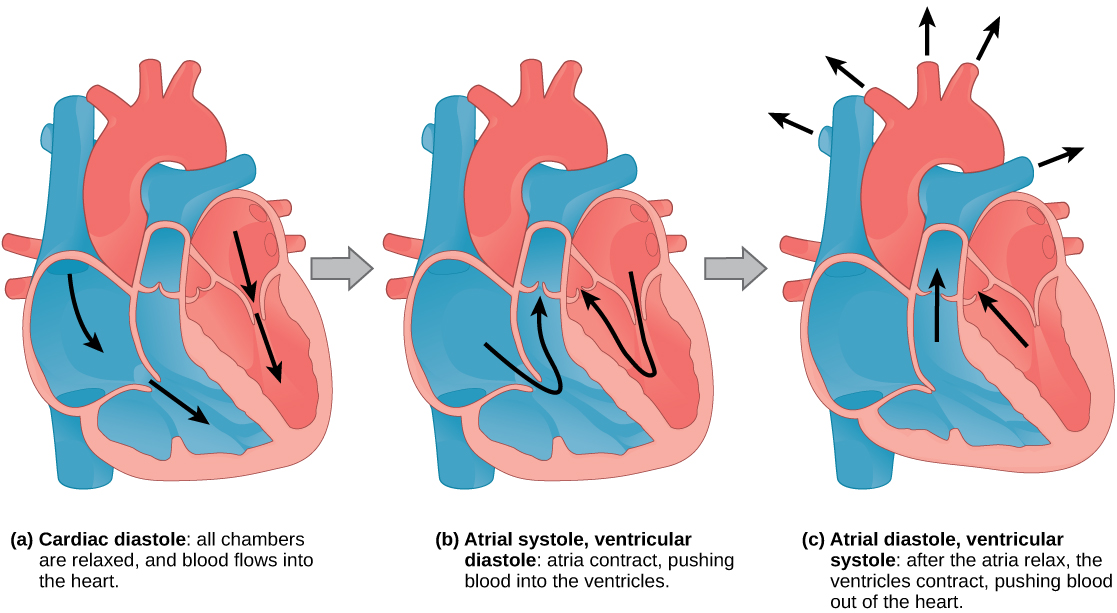
\includegraphics[width=14cm]{heart.jpg}
\centering
\caption{Heart contractions during a cardiac cycle}
\end{figure}
\

Mechanical vibrations reflect the turbulence that occurs when heart valves close. Traditionally, a stethoscope is used in cardiac auscultation to listen to these sounds that provide important acoustic information regarding the health condition of the heart. \cite{4}
\\

Phonocardiography, is a diagnostic technique that creates a graphic record, called phonocardiogram, of the sounds and murmurs produced by the contracting heart. The phonocardiogram is obtained either with a chest microphone or with a miniature sensor in a small tubular instrument that is introduced through the blood vessels into one of the heart chambers. The phonocardiogram usually supplements the information obtained by listening to body sounds with a stethoscope (auscultation) and is of special diagnostic value when performed simultaneously with measurement of the electrical properties of the heart (electrocardiography) and pulse rate.\cite{6}
\\

The time-frequency analysis of the PCG signals permits detecting and characterizing abnormal murmurs or extra sounds (systole or diastole) in the diagnosis of heart disease. In this study, we analyze normal, murmur and extra heart sounds recordings, separating them from artifacts. Most often, the symptoms of cardiovascular diseases become worse over time and detecting them with noninvasive techniques in early stages is crucial.
\\

The correlation among the phonocardiogram and the biological phenomenon is presented in the following diagram:

\begin{figure}[h]
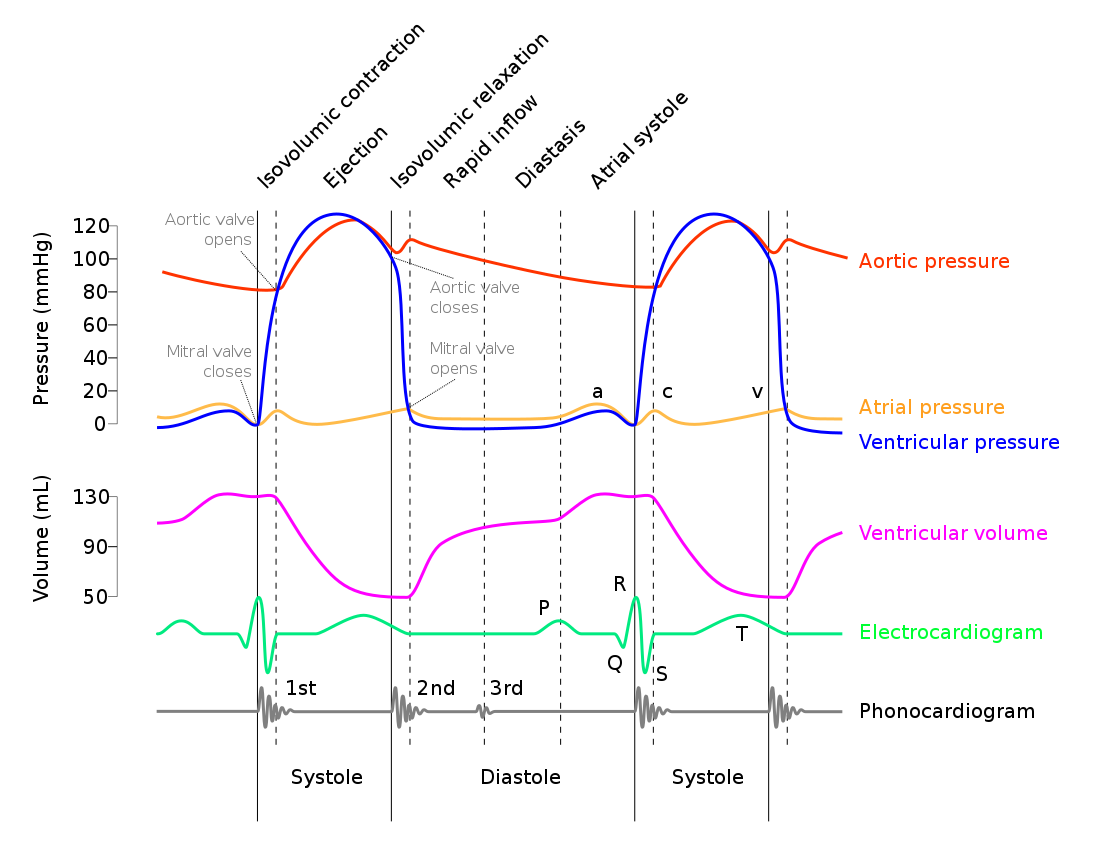
\includegraphics[width=15cm]{Wiggers_Diagram_2.png}
\centering
\caption{The Wiggers Diagram illustrating the cardiac cycle}
\end{figure}
\
\\
\
\\
\
\\
\
\\
\

\textbf{Heart murmur}
\\

Heart murmurs are heart sounds produced when blood flows across one of the heart valves that are loud enough to be heard with a stethoscope. Heart murmurs are most frequently categorized, into systolic murmurs and diastolic murmurs, differing in the part of the heartbeat on which they can be heard. There are also, continuous murmurs cannot be directly placed into either category.
\\

Systolic murmurs are due to blood flow through the semilunar valves. They occur at the start of blood ejection — which starts after S1 — and ends with the cessation of the blood flow — which is before S2. Diastolic murmurs start after S2 and end before S1. Many involve stenosis of the atrioventricular valves or regurgitation of the semilunar valves. \cite{10}
\\
\
\\

\textbf{Heart arrhythmia and extra beats}
\\

Heart arrhythmia (also known irregular heartbeat) is a group of conditions in which the heartbeat is irregular, too fast, or too slow. There are four main types of arrhythmia: extra beats, supraventricular tachycardias, ventricular arrhythmias, and bradyarrhythmias. Extra beats, part of our dataset, come in two different types, premature atrial contractions and premature ventricular contractions. Often they cause no symptoms but may present with fluttering in the chest or a skipped beat. \cite{11}
\\


\addcontentsline{toc}{section}{I.2. Previous work}
\section*{I.2. Previous work}
\

Many studies have been done on phonocardiogram signal so far. The research on this topic increased nowadays due to improvement in signal processing techniques and new methods in big data analysis. A summary of the most important results obtained with the Classifying Heart Sounds PASCAL Challenge dataset can be found here [24-25].
\\

The Classifying Heart Sounds Workshop 2012 is the first international workshop to focus on the use of statistical machine learning techniques to segment and classify real-world heart audio. The challenge for this workshop was to create a first level of screening of cardiac pathology both in a Hospital environment by a doctor (using a digital stethoscope) and at home by the patient (using a mobile device). 
\\

The problem is of particular interest to machine learning researchers as it involves classification of audio sample data, where distinguishing between classes of interest is non-trivial. Success in classifying this form of data requires extremely robust classifiers. 
\\

\begin{figure}[h]
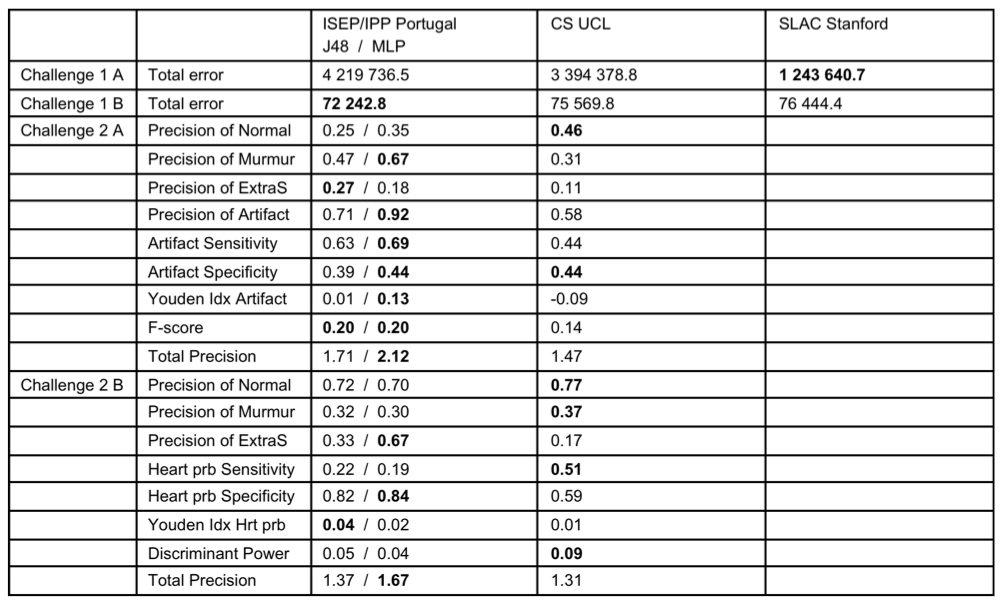
\includegraphics[width=16cm]{challengeresults.png}
\centering
\caption{A summary of the results of the three finalists from their approaches}
\end{figure}
\
\\
\

The first team uses, after the segmentation, the J48 and MLP algorithms (using Weka) to train and classify the computed features. The UCL team exploits domain knowledge and compares the features of heartbeat before and after dropping out extra peaks and the smallest interval. By doing so they try to minimize the negative effect of noise. [24-25] In the literature there are other proposed ways to tackle this challenge: partial least squares regression, neural networks and convolution neural networks.
\\

Other models for classifying the heart sounds can be found \cite{27}, where the best general accuracy obtained was $93,18 \%$ for all the classes. The model proposed is a neural network.


\newpage



\addcontentsline{toc}{chapter}{II. Methodology and research methods}
\chapter*{II. Methodology and research methods}

\addcontentsline{toc}{section}{II.1. CRISP-DM Methodology}
\section*{II.1. CRISP-DM Methodology}
\

Cross-industry standard process for data mining, commonly known by its acronym CRISP-DM, is a data mining process model that describes commonly used approaches used to tackle problems. The current process model for data mining provides an overview of the life cycle of a data mining project. It contains the phases of a project, their respective tasks, and the relationships between these tasks. At this level, it is not possible to identify all relationships. Relationships could exist between any data mining tasks depending on the goals, the background, the interest of the user and on the data. \cite{12}
\\

The life cycle of a data mining project consists of six phases, shown in the next figure. The sequence of the phases is not fixed. Moving back and forth between different phases can be required. The outcome of each phase determines which phase has to be performed next. The arrows indicate the most important and frequent dependencies between phases.
\\

\begin{figure}[h]
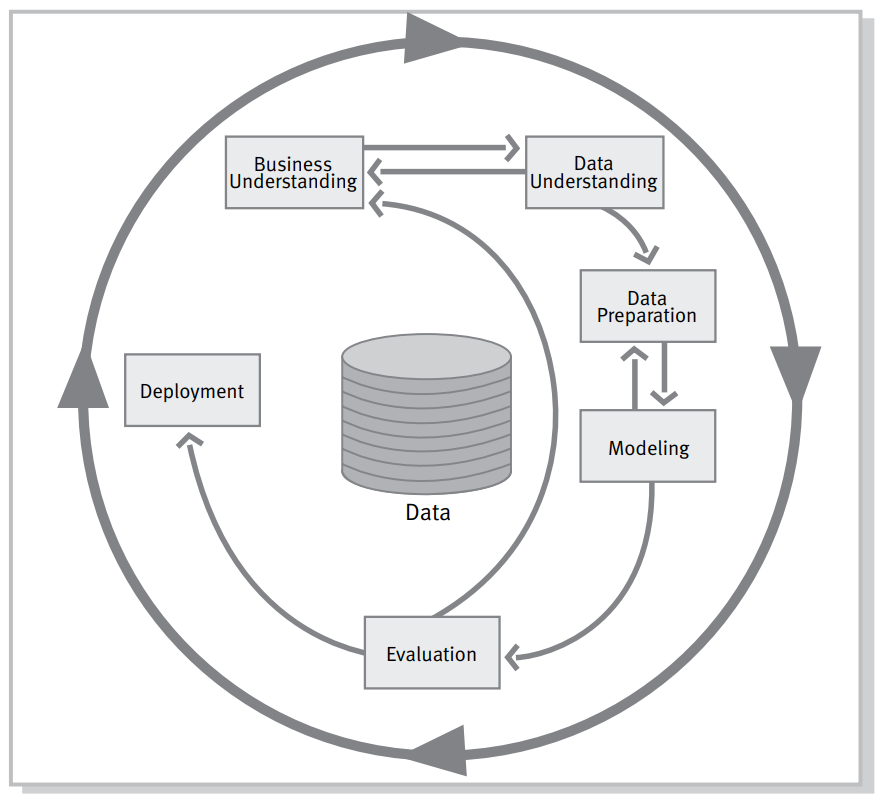
\includegraphics[width=8cm]{crisp.png}
\centering
\caption{Phases of the CRISP-DM model}
\end{figure}
\


\textbf{Business understanding}

\

The initial phase main purpose is understanding the project objectives and requirements from a business perspective, analyzing the available resources, and then converting this knowledge into a data mining problem definition, and a plan designed to achieve all the objectives. 
\\

For our study the main objective is to predict with a high rate of trust if a person has arrhythmia or murmurs through a phonocardiogram. The resources available for us are a dataset of different types of recordings, a graphic card GeForce GTX 1050 (2GB) and a Intel(R) Core(TM) i7-7700HQ CPU @ 2.80GHz. Our initial goal would be to get a good accuracy at test.
\\

\textbf{Data understanding}

\

The data understanding phase starts with an initial data collection and proceeds with activities that can give insides about the data, to identify data quality problems, or to detect interesting subsets to form hypotheses for hidden information.
\\

Our dataset has been gathered from two sources. All the files are .wav files with lengths between 1 second and 30 seconds and two frequencies: 44100 Hz and 4000 Hz. We also have examples of recordings there are not heartbeats, but artifacts.
\\

\textbf{Data preparation}

\

This phase covers all activities to construct the final dataset (data that will be used for creating the model) from the initial raw data. Tasks representative for the data preparation phase include table, record, and attribute selection as well as transformation and cleaning of data for modeling tools.
\\

In this phase we normalized each recording using the Frobenius norm and after this, using a peak detection algorithm, we identified the sounds S1 and S2 in each recording. We searched for the peaks starting with second 0,5 and ended at len(rec) - 0,5 seconds. For each peak we sliced a 1 second piece of the record, obtaining multiple one second recordings. In order to get a better accuracy through multiplying the data we used a sliding window technique.
\\

\textbf{Modeling}

\

In this phase, various modeling techniques are selected and applied, and their parameters are calibrated to optimal values. Usualy, there are several techniques for the same data mining problem type. Some techniques have specific requirements on the form of data.
\\

The models we created are one Convolutional Neural Networks that classifies each record in one of the four classes, and the second model uses a Multi-Task Learning technique in Convolutional Neural Networks.

\textbf{Evaluation}

\

At this stage in the project you have built a model (or models) that appears to have good quality, from a data analysis perspective. Before proceeding to final deployment of the model, it is important to evaluate the model, and review the steps executed to construct the model, to be certain it achieves the business objectives.
\\

The metrics we used for evaluating the models is te accuracy of the test dataset. Other metrics that we used are the validation dataset accuracy, the value of the loss function, the sensitivity and the specificity.
\\

\textbf{Deployment}

\

Creation of the model is not the end of the project. Even if the purpose of the model is to increase knowledge of the data, the knowledge gained will need to be organized and presented in a way that is useful to the users. Depending on the requirements, the deployment phase can be as simple as generating a report or as complex as implementing an application from scratch. In many cases it will be the customer who will carry out the deployment steps. 



\begin{figure}[h]
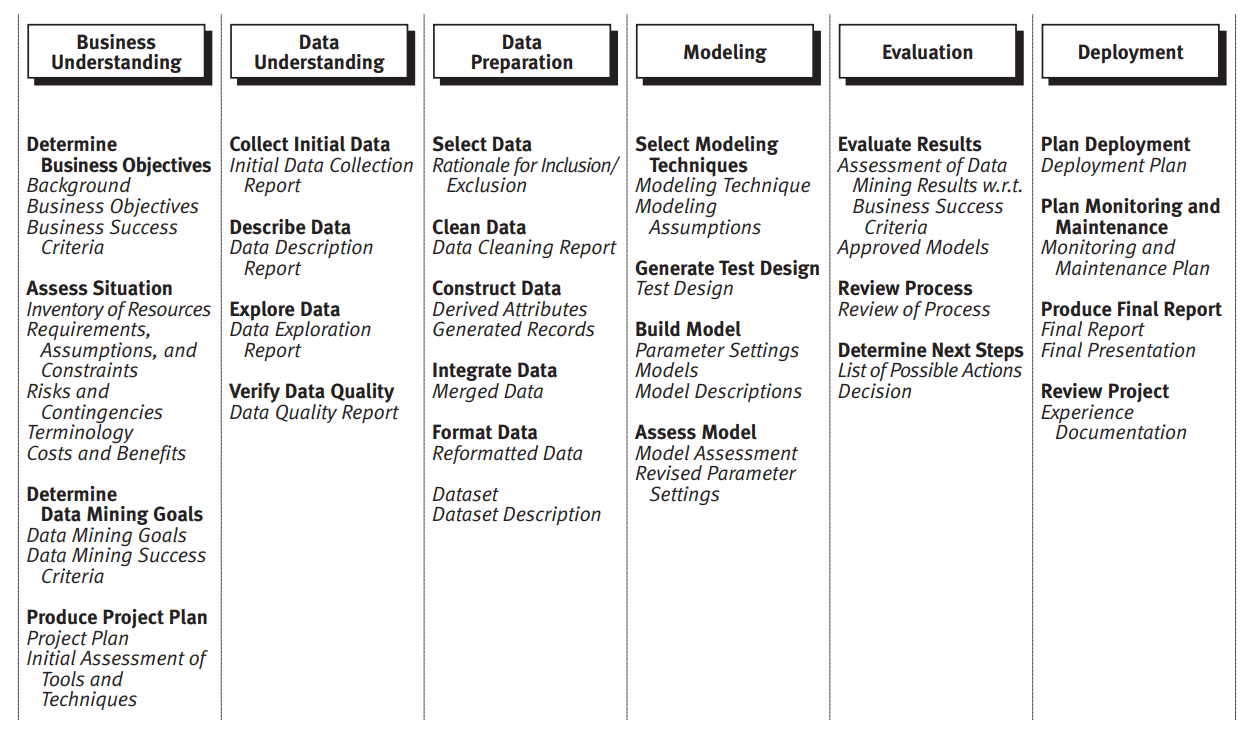
\includegraphics[width=16.2cm]{crispt.png}
\centering
\caption{Generic tasks and outputs of the CRISP-DM model}
\end{figure}
\

In the next sections we will detail some of the most important and time consuming phases of the project, detailing the mathematical and biological background for each stage.
\
\newpage

\addcontentsline{toc}{section}{II.2. Data understanding and preparation}
\section*{II.2. Data understanding and preparation}
\

\addcontentsline{toc}{subsection}{II.2.1. Data Description and Selection}
\subsection*{II.2.1. Data Description and Selection}

\

The dataset is split into two sources, A and B. The recordings from the A dataset are gathered from the general public via the iStethoscope Pro iPhone app. The second dataset, B, is collected from a clinic trial in hospitals using the digital stethoscope DigiScope. Most information in heart sounds is contained in the low frequency components, with noise in the higher frequencies. \cite{2}
\\

The audio files have varying lengths, between 1 second and 30 seconds (some have been clipped to reduce excessive noise and provide the salient fragment of the sound). The two datasets differ in number, frequency and other proprieties of the .wav files.
\\

A file with the \verb|.wav| file extension is a Waveform Audio file. This is a standard audio format. It is an extension of the bitstream format Resource Interchange File Format (\verb|RIFF|). \verb|WAV| is similar to \verb|AIFF| and \verb|8SVX| files.
\\

\textbf{Dataset A}

\

The recordings from this dataset are gathered using the iStethoscope Pro iPhone app. All of them are represented with on a 705  bitrate, through a mono channel. The samples rate is 44100 Hz. The following types of heartbeats are recorded and labeled:

\

Atraining\_normal 14Mb 31 files
\

Atraining\_murmur 17.3Mb 34 files
\

Atraining\_extrahs 6.9Mb 19 files
\

Atraining\_artifact 22.5Mb 40 files

\

\textbf{Dataset B}

\

The recordings from this dataset are gathered using DigiScope. All of them are represented with on a 705  bitrate, through a mono channel. The samples rate is 4000 Hz. The following types of heartbeats are recorded and labeled:

\

Btraining\_normal (containing sub directory Btraining\_noisynormal) 13.8Mb 320 files
\

Btraining\_murmur (containing sub directory Btraining\_noisymurmur) 5.3Mb 95 files
\

Btraining\_extrasystole 1.9Mb 46 files
\\


\addcontentsline{toc}{subsection}{II.2.2. Preprocess Data}
\subsection*{II.2.2. Preprocess Data}

\

Data preparation is the process of getting data ready for applying different models. During data preparation, we have to take the data that is stored in raw form and transform it so that it can be effectively used by machine learning algorithms. 
\\


\addcontentsline{toc}{subsubsection}{II.2.2.a. Frames retrieval}
\subsubsection*{II.2.2.a. Frames retrieval}

\

In order to use the whole dataset (A and B) we need to transform the recordings at the same frame-rate. We choose 16000 Hz in order not to loose much information from the B dataset, and to enhance the A dataset with more values for the same unit of time. 
\\

We used \verb|ffmpeg| command to transform all the data. With a bash script we iterated through the \verb|.wav| files and changed all of them at 16000 Hz. \cite {5}
\begin{center}
\begin{tabular}{c}
\begin{lstlisting}
ffmpeg  -i {file} -ar 16000 {file} -y
\end{lstlisting}
\end{tabular}
\end{center}

After all the recording had the same meta-data (except the length), we iterated through the dataset and parse each file in Python, in order to process them. We use the wave library to open the recordings and read them frame by frame. We obtained arrays of length equal with the duration in time of the recording multiplied with the framerate (16000 Hz).
\\

An audio frame, or sample, contains amplitude (loudness) information at that particular point in time. To produce sound, tens of thousands of frames are played in sequence to produce frequencies.
\\

In our case there are 16000 frames/samples per second. Each of those frames contains 16-bits of resolution, allowing precise representations of the sound levels. When we use the sound module in Python to get a frame, it will be returned as a series of hexadecimal characters, two characters for 16-bit mono.

\begin{center}
\begin{tabular}{c}
\begin{lstlisting}
b'\x0e\x00\x11\x00\x0e\x00\x00\x00\x02\x00\x0b\x00\xfe\xff'
\end{lstlisting}
\end{tabular}
\end{center}

We unpack the bytestring by using the struct library in Python. struct requires a format string based on C format characters, so we use the signed format that corresponds to 2 bytes; according to the C format characters, we should use the format character 'h'.
\\

A slight trick in the struct library is that it wants its format string to exactly match the expected size, so we have to multiply the format character 'h' by the number of frames in the bytestring.

\begin{center}
\begin{tabular}{c}
\begin{lstlisting}
samples = struct.unpack('h' * f.getnframes(), frames)
#frames holds the bytestring representing the audio frames
\end{lstlisting}
\end{tabular}
\

(14, 17, 14, 0, 2, 11, -2) - for the previous example
\end{center}


\addcontentsline{toc}{subsubsection}{II.2.2.b. Ploting}
\subsubsection*{II.2.2.b. Ploting}

\

For plotting the recordings to better visualize the samples from the dataset we need a different tool. To get the timing, we'll grab the sampling rate from the wave object. In order to get better conclusions we plotted the whole record.
\\

We have here some examples of the records with normal, murmur and extrasystole sounds, but also some examples of artifacts.
\


\begin{figure}[H]
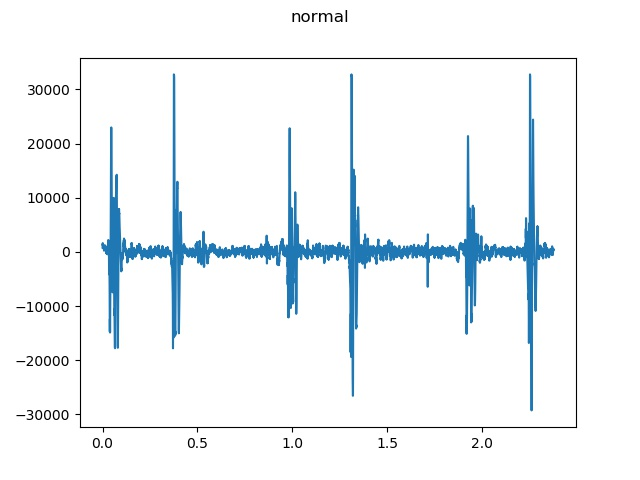
\includegraphics[width=11cm]{img/beforenorm/normal__106_1306776721273_C2.jpg}
\centering
\caption{Example of normal heartbeat phonocardiogram}
\

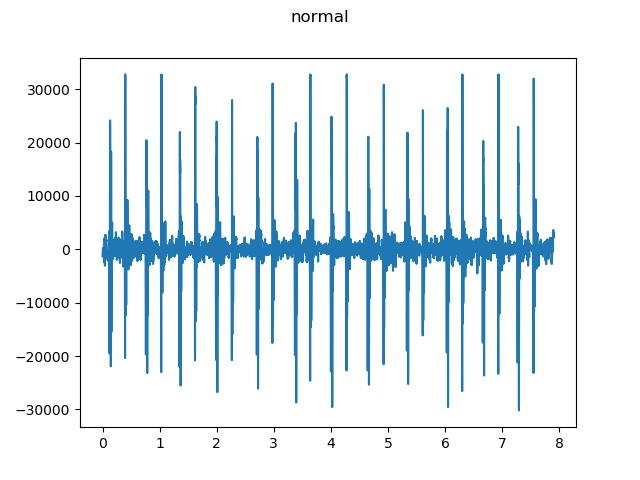
\includegraphics[width=11cm]{img/beforenorm/normal__128_1306344005749_B.jpg}
\centering
\caption{Example of normal heartbeat phonocardiogram}
\end{figure}
\

\begin{figure}[H]
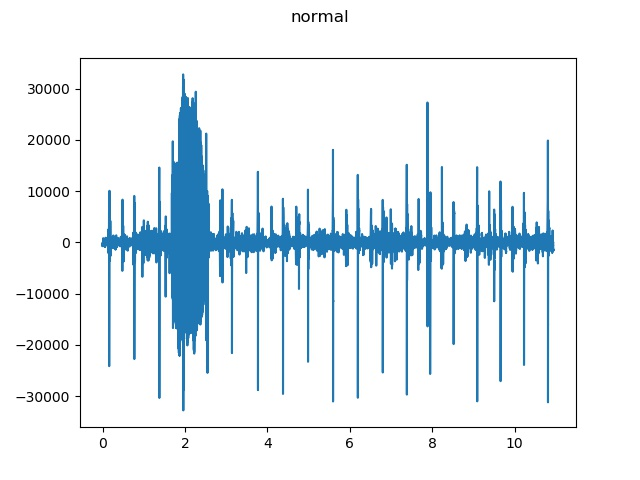
\includegraphics[width=9cm]{img/beforenorm/normal_noisynormal_127_1306764300147_D1.jpg}
\centering
\caption{Example of noisy normal heartbeat phonocardiogram}
\

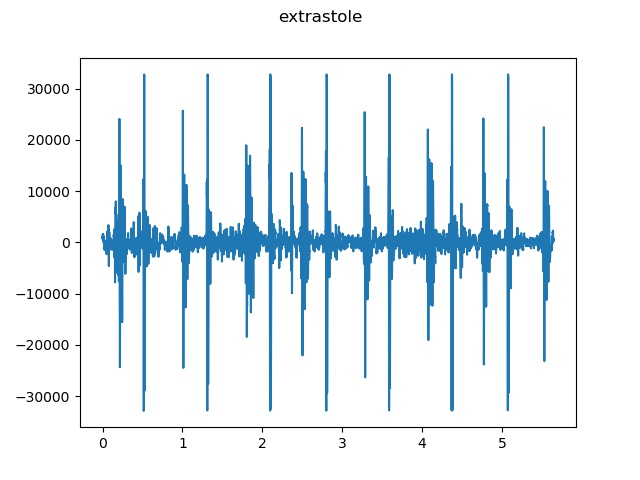
\includegraphics[width=9cm]{img/beforenorm/extrastole__209_1308162216750_D.jpg}
\centering
\caption{Example of extrasystole heartbeat phonocardiogram}
\

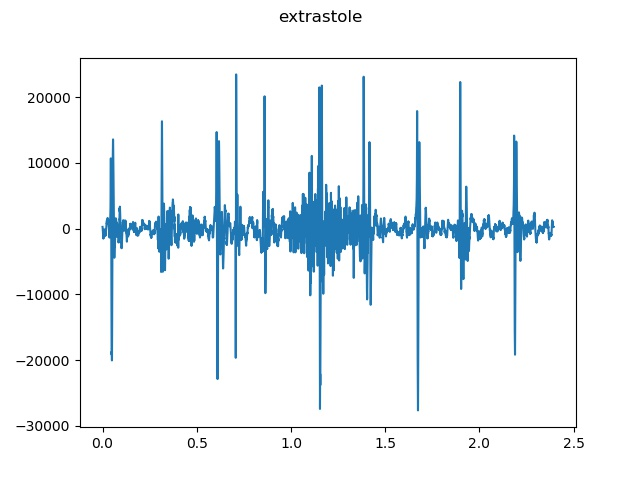
\includegraphics[width=9cm]{img/beforenorm/extrastole__154_1306935608852_D2.jpg}
\centering
\caption{Example of extrasystole heartbeat phonocardiogram}

\end{figure}
\

\begin{figure}[H]
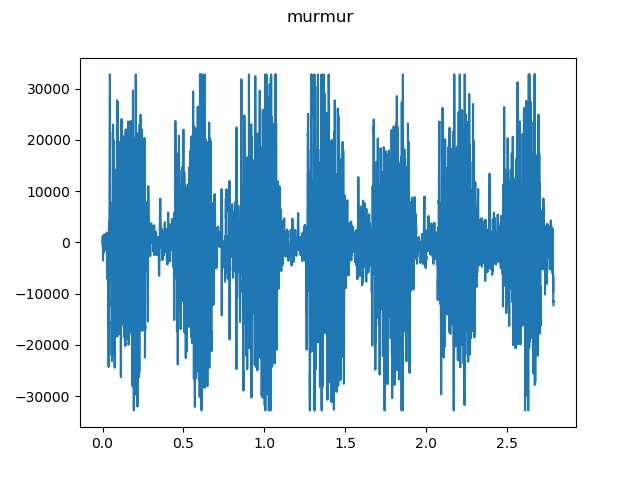
\includegraphics[width=9cm]{img/beforenorm/murmur__171_1307971016233_D.jpg}
\centering
\caption{Example of murmur heartbeat phonocardiogram}
\

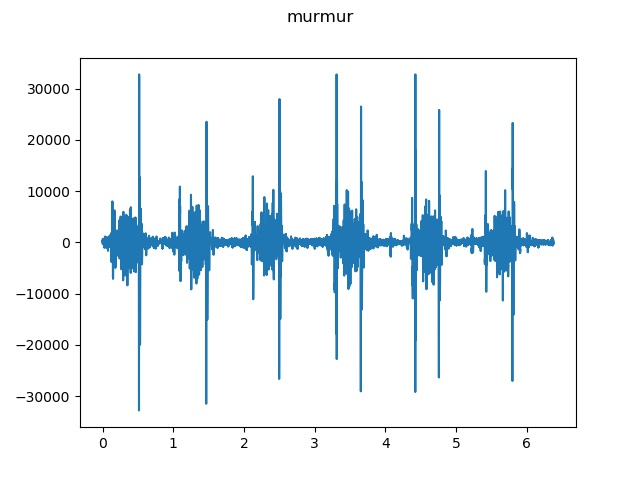
\includegraphics[width=9cm]{img/beforenorm/murmur__242_1309197394064_B.jpg}
\centering
\caption{Example of murmur heartbeat phonocardiogram}
\

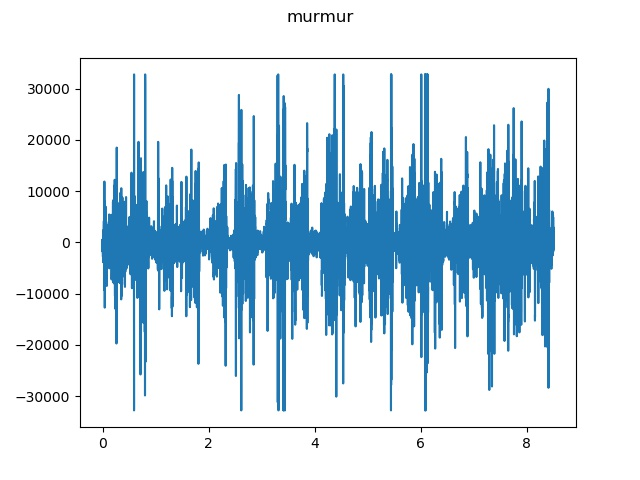
\includegraphics[width=9cm]{img/beforenorm/murmur_noisymurmur_162_1307101835989_B_1.jpg}
\centering
\caption{Example of noisy murmur heartbeat phonocardiogram}
\end{figure}
\

\addcontentsline{toc}{subsubsection}{II.2.2.c. Peak Analysis}
\subsubsection*{II.2.2.c. Peak Analysis}

\

Another step of the data preprocessing phase is the peak detection. Identifying and analyzing peaks (also  called spikes) in a given time-series  is important in many applications, because peaks are useful topological  features of a time-series. In phonocardiograms, a peak is one of the sounds that the heart produces. \cite{17}
\\

This problem was encountered in many signal processing applications. Up to
now, many different methods have been developed and the window-threshold technique is the one we implemented. 

\begin{minted}{Python}
def is_peak (x, left, right):
	return np.amax(left) < x and np.amax(right) < x

def get_peaks(samples):
	std = np.std(samples)
	for i in range(len(samples)):
		if samples[i] > std * 2.8:
			if is_peak(samples[i], 
				   samples[i - Cframerate // 5 : i], 
				   samples[i + 1 : i + Cframerate // 5]):
				sol.append(i)
	return sol
\end{minted}
\

The algorithm presented has as input the array that represents a whole recording and the output is a list that has all the peaks positions in time.
\\

We need the variation of the dataset in order to create a threshold for selecting the possible heartbeat. Because of the noise that each recording has, we need to approximate where do most of the heartbeats start. The value we picked is 2.8 multiplied with one standard deviation. In this interval we have about 99\% of the data, and the other values will be tested if they are peaks. \cite{21}
\\

We will check for each feasible solution, if it satisfies our criteria. In order to call a frame, peak, it should be the greatest value in the window we created. The window size is 0.2 seconds, and we test if the current value is the peak of this interval. When we find a value suitable, we append it to the list of solutions.
\

\begin{figure}[H]
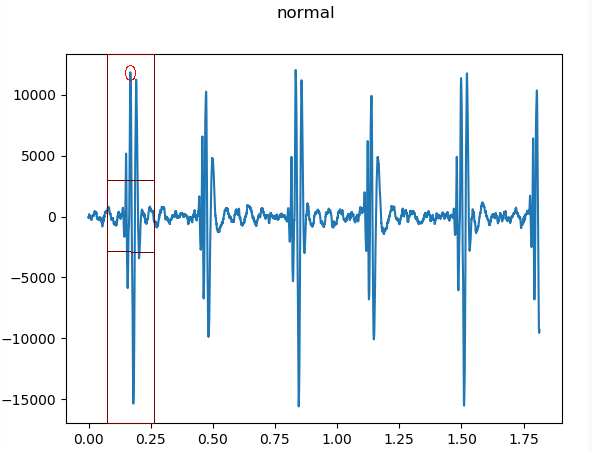
\includegraphics[width=9cm]{n1a.png}
\centering
\caption{Identifying the first heartbeat sound in a record. In a window of size 0.2 seconds we found the value that is the peak and respects all the conditions}
\

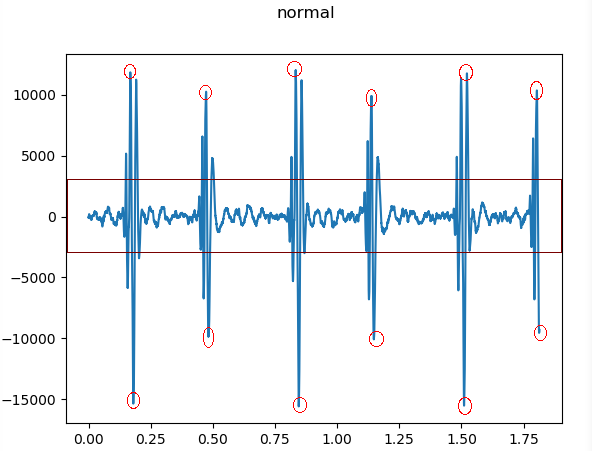
\includegraphics[width=9cm]{n1c.png}
\centering
\caption{All detected heartbeat sounds in a record. All absolute values of the peaks are greater than $2.8 * std(rec)$}
\end{figure}
\

\addcontentsline{toc}{subsection}{II.2.3. Data Transformations}
\subsection*{II.2.3. Data Transformations}

\

The final step of the data preparation phase is to transform the processed data. The specific algorithm we will be working with and the knowledge of the problem domain influence this step. The following data transformations were applied on our dataset, while scaling, attribute decomposition and attribute aggregation are the most common techniques used. This step is also referred to as feature engineering.
\\


\addcontentsline{toc}{subsubsection}{II.2.3.a. $L^2$ norm}
\subsubsection*{II.2.3.a. $L^2$ norm}

\

In this point we have 585 arrays of different lengths that contain negative and positive values that represent the amplitude of the recording in a unit of time. These values are between $[-40000,40000]$, and so they are difficult to work with, because the result of different computations can exceed the limits.
\\

A solution for this problem would be to normalize all the arrays. We choose to use the $L^2$ norm for this task. The value of the $L^2$ norm is between $[L^{\infty}=max_{x_i \in rec}(x_i),L^1=\sum_{x_i \in rec}(x_i)]$, so the values for each frame will be divided by a value grater than it. \cite{15} This means that all the values will be much smaller than 1 (or -1). In order not to loose precision we multiplied the values with 100. To compute the $L^2$ norm we used the Numpy library.

\begin{minted}{Python}
fac_norm = np.linalg.norm(samples)
samples = (samples / fac_norm) * 100
\end{minted}

Next we will present the mathematical background for computing the norms.
\\

Given an $n$-dimensional vector $x \in \mathbb{R}^n$, the $L^2$ norm, also called Euclidean norm, is captured by the formula :

\[
x = \begin{bmatrix}
    x_1\\
    x_2\\
    \cdots\\
    x_n
\end{bmatrix} \in \mathbb{R}^n,
\]
\
\[
\parallel x \parallel _2 = \sqrt{x_1^2+x_2^2+\cdots+x_n^2}
\]

The $L^2$ norm is a particular case for the $p-$norm, where $p=2$. \cite{16}
\[
\parallel x \parallel _p = \sqrt[p]{|x_1|^p+|x_2|^p+\cdots+|x_n|^p}
\]
\
After we divided by the norm, we multiplied the values with 100, and we obtained the exact values heartbeats with values greater than 1, or lower than -1.

\begin{figure}[H]
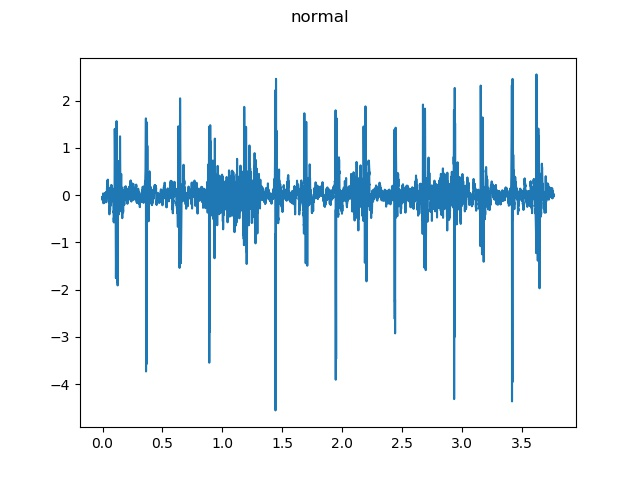
\includegraphics[width=9cm]{img/normal__113_1306244002866_D.jpg}
\centering
\caption{Heartbeat phonocardiogram normalized}
\

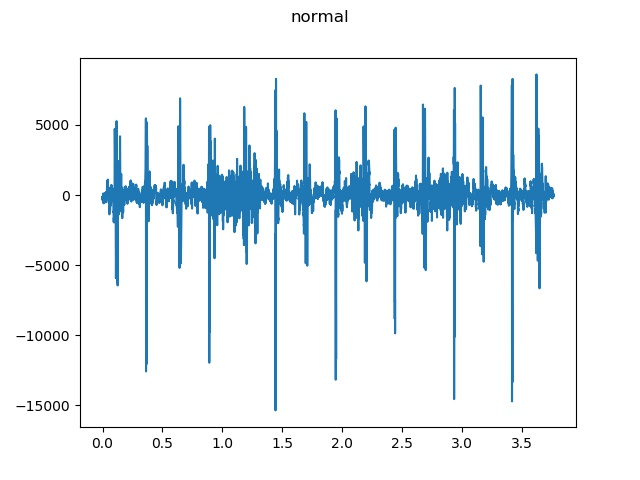
\includegraphics[width=9cm]{img/beforenorm/normal__113_1306244002866_D.jpg}
\centering
\caption{Heartbeat phonocardiogram before normalization}
\end{figure}
\


\addcontentsline{toc}{subsubsection}{II.2.3.b. Sliding window for data selection}
\subsubsection*{II.2.3.b. Sliding window for data selection}

\

A sliding window is a sublist that runs over an underlying collection. After we have the list of the peaks from our recordings, we sliced one second of the audio file, centered in each peak. We choose this approach according to the results obtained by \cite{14}.
\\

In order to increase the accuracy of our models, we tried to move this window with 0,0025 seconds and 0.005 seconds, left and right. This way, from only one array of values we got now five new entries in our dataset. This method for multiplying the data we use as input for the classifiers, helps better generalize the rules for obtaining good results. \cite{19}


\begin{figure}[H]
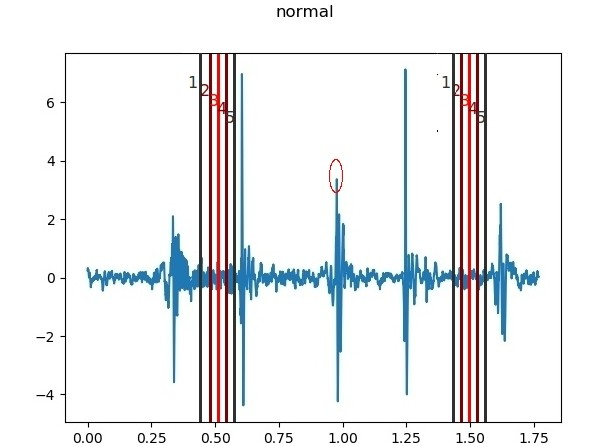
\includegraphics[width=9cm]{sw.jpg}
\centering
\caption{The 5 segments of audio recording that are centered in the peak pointed}
\end{figure}
\


\addcontentsline{toc}{subsubsection}{II.2.3.c. Feature extraction}
\subsubsection*{II.2.3.c. Feature extraction}

\

Given a set of samples on which a decision should be made, a feature is a value that would possibly be different among those samples and discriminate one sample from another. This decision may be, as in our case, to classify the sample to a finite set. Feature extraction is the process of collecting discriminatory information from a set of samples.
\\

The CNN we built have as input the raw recordings, but in the multi task learning model, for classifying the extrastole, we compared the AdaBoost Classiffier and a decision tree. In order to be able to use this classifiers, we needed real values that can  After features are extracted, Classification is performed based on the selected features. The performance of classifier depends on both how good the signals are pre-processed and how good the features are extracted. \cite{14}
\\

In this thesis a total of 11 features from time domain, frequency domain and statistical features were extracted that could have potential to discriminate among the extrastole and other(normal and murmur) signals. The features in the whole signal have been extracted in order to deal with the situations of extrasystole sounds. \cite{7}
\

\begin{minted}{Python}
def features(arr):
	peaks_list = get_peaks (arr)
	dists = distances (peaks_list)
	
	getInfo = lambda x, f1, f2: [f1(x), f2(x)]
	
	sol += getInfo(dists, np.mean, np.std)
	sol += getInfo(peaks_list, np.mean, np.std)
	sol += getInfo(dists, np.min, np.max)
	sol += getInfo(peaks_list, np.min, np.max)
	sol += getInfo(arr, np.mean, np.std)
	sol.append(len(peaks_list))
	
	return sol
\end{minted}
\

The potential seen in these features and hence the reason for evaluating these features is explained further.
\\

\begin{longtable}[!h]{ | m{0.6cm} | m{3cm}| m{3.2cm} | m{6.5cm} | } 
\hline
No.& Feature & Feature domain & Details \\ 
\hline\hline
1 & Peak Frequency & Frequency domain & It shows the frequency at which the peak amplitude occurs. Since the extra sounds appear between the intervals of regular sounds, it could have been a potential feature. \\ 
\hline
2 & Peak Frequency Standard Deviation & Frequency domain \ & It quantifies the amount of dispersion of the peak occurrences. The existence of extra sounds should indicate a greater value. \\ 
\hline
3 & Peak Amplitude & Time domain &  The mean peak amplitude shows the peak value of the signal. The extra sounds and normal signals can vary in amplitude so this feature has potential. \\ 
\hline
4 & Peak Amplitude Standard Deviation & Time domain & If the standard deviation of the peak amplitude is greater, it means that the sounds have different intensity, and this can be a sign of extra sounds. \\ 
\hline
5 & Minimum Peak Distance & Frequency domain & It represents the smallest distance between 2 consecutive heartbeat sounds identified in the record. If this value is small it can be the distance between an extra sound and a regular beat. \\ 
\hline
6 & Maximum Peak Distance & Frequency domain & It represents the longest time between 2 consecutive heartbeat sounds identified in the record. This value can show if there is an abnormal distance between consecutive sounds.  \\ 
\hline
7 & Minimum Peak Amplitude & Time domain & Normal heart sounds have about the same amplitude (assuming that that systole is not very shorter than diastole). An extra sound is a variation of these values, so a small value can be an extra sound. \\ 
\hline
8 & Maximum Peak Amplitude & Time domain & Normal heart sounds have about the same amplitude (assuming that that systole is not very shorter than diastole). An extra sound is a variation of these values, so a big value can represent an extra sound. \\ 
\hline
9 & Mean Amplitude & Time domain & The mean amplitude of the one second window can be correlate with the standard deviation of all the values.\\ 
\hline
10 & Standard Deviation Amplitude & Time domain &  If the dispersion of all the values in the one second window is big than it means that we have more values that have different values than the mean. \\ 
\hline
11 & Number of Peaks & Statistical & The only discrete feature we used for classification, the number of peaks in one second represents the number of heart sounds we identified in this interval.\\ 
\hline

\caption{List of Features Extracted for Classification}
\end{longtable}

All the features are calculated from the PCG signals. Two algorithms for Attribute Evaluation are applied on the feature set to find the most significant features. The results are presented in the next chapter. 
\
\newpage

\addcontentsline{toc}{section}{II.3. Classification Models}
\section*{II.3. Classification Models}

\

As the first step in modeling, we select the actual modeling technique that is to be used. Out picks are CNN and AdaBoost. The models we created and used for testing are presented in the following subsections.


\addcontentsline{toc}{subsection}{II.3.1. Multi-Class CNN}
\subsection*{II.3.1. Multi-Class CNN}

\

Using the normalized and segmented sound recordings, a CNN is trained to extract features and construct a classification function. The CNN consists of 6 layers, namely convolution layers and fully connected layers. \cite{18}
\\

First, the convolution layer extracts high level (abstracted) features by sequentially transforming raw input data into high-level abstract features. The convolution layer contains a non-linear activation function, kernel regularizer and max pooling layers. 
\\

The non-linear activation function is Relu and is used to increase the representability of a network (increase the fitness of a model). We used the L2 regularization. The max pooling layer selects the maximum value among its neighbors to reduce noise and extract abstract features. After having gone through the convolution layer, the features are autonomously extracted from the segmented signals.
\\

Fully connected layers output values for classification predictions by linearly combining the features extracted from convolutions layers and having the combined values go through non-linear activation functions. The last layer uses the softmax activation function. As one segmented signal goes through the convolution and fully-connected layers, the features are extracted and used to classify the signal, respectively.
\\

After an architecture of CNN is designed, the parameters of CNN have been trained by back propagation algorithm with the categorical crossentropy loss function and mini-batch learning using training data. We use Keras to construct and train our model.
\\

\begin{minted}{Python}
Layer (type)                 Output Shape              Param #   
=================================================================
conv1d_1 (Conv1D)            (None, 15991, 12)         132       
_________________________________________________________________
max_pooling1d_1 (MaxPooling1 (None, 3198, 12)          0         
_________________________________________________________________
flatten_1 (Flatten)          (None, 38376)             0         
_________________________________________________________________
dense_1 (Dense)              (None, 500)               19188500  
_________________________________________________________________
dense_2 (Dense)              (None, 100)               50100     
_________________________________________________________________
dense_3 (Dense)              (None, 20)                2020      
_________________________________________________________________
dense_4 (Dense)              (None, 3)                 63        
=================================================================
Total params: 19,240,815
Trainable params: 19,240,815
\end{minted}




\addcontentsline{toc}{subsection}{II.3.2. Multi-Task Learning}
\subsection*{II.3.2. Multi-Task Learning}

\

In Machine Learning, we typically care about optimizing for a particular metric. By sharing representations between related tasks, we can enable our model to generalize better on our original task. This approach is called Multi-Task Learning (MTL).
\\

In the context of Deep Learning, multi-task learning is typically done with either hard or soft parameter sharing of hidden layers. Our approach uses soft parameter sharing. In soft parameter sharing on the other hand, each task has its own model with its own parameters. MTL is a natural fit in situations where we are interested in obtaining predictions for multiple tasks at once, so this method can be applied to our problem. We split the multi class-decision in three different tasks. \cite{23}

\addcontentsline{toc}{subsubsection}{II.3.2.a. Neural Network Normal heartbeat}
\subsubsection*{II.3.2.a. Neural Network Normal heartbeat}

\

For deciding weather a heartbeat is normal or not, we trained a CNN to extract features and construct a classification function. The CNN consists of 6 layers.
\\

First, the convolution layer extracts high level (abstracted) features with 4 filters. The convolution layer uses Relu as activation function, kernel regularizer and max pooling layers. We used the L2 regularization. The max pooling layer selects the maximum value among its neighbors. The fully connected layers linearly combine the features extracted from convolutions layers. The last layer uses the softmax activation function. As one segmented signal goes through the convolution and fully-connected layers, the features are extracted and used to classify the record.
\\

The parameters of CNN have been trained by back propagation algorithm with the Kullback Leibler divergence loss function and mini-batch learning using training data.
\\

Consider two probability distribution $P$ and $Q$ over the same domain $X$. The Kullbach-Leibler divergence is computed in the following way.
$$ D_{KL}(P, Q) = \sum_{x \in X} P(x) log \frac{P(x)}{Q(x)} $$
\

\begin{minted}{Python}
Layer (type)                 Output Shape              Param #   
=================================================================
conv1d_1 (Conv1D)            (None, 15991, 4)          44        
_________________________________________________________________
max_pooling1d_1 (MaxPooling1 (None, 3198, 4)           0         
_________________________________________________________________
flatten_1 (Flatten)          (None, 12792)             0         
_________________________________________________________________
dense_1 (Dense)              (None, 500)               6396500   
_________________________________________________________________
dense_2 (Dense)              (None, 100)               50100     
_________________________________________________________________
dense_3 (Dense)              (None, 20)                2020      
_________________________________________________________________
dense_4 (Dense)              (None, 2)                 42        
=================================================================
Total params: 6,448,706
Trainable params: 6,448,706
\end{minted}



\addcontentsline{toc}{subsubsection}{II.3.2.b. Neural Network Murmur heartbeat}
\subsubsection*{II.3.2.b. Neural Network Murmur heartbeat}

\

The CNN used for classifying murmur heartbeats is trained to extract features and construct a classification function. The CNN consists of 6 layers, namely convolution layers and fully connected layers.
\\

The convolution layer extracts abstract features from raw input data. The convolution layer is formed from Relu activation function, L2 regularization and max pooling layers.The max pooling layer selects the maximum value among its neighbors to reduce noise and extract abstract features.
\\

Fully connected layers output values for classification predictions by linearly combining the features extracted from convolutions layers. The last layer uses the softmax activation function. As one segmented signal goes through the convolution and fully-connected layers, the features are extracted and used to classify the signal, respectively.
\\

After an architecture of CNN is designed, the parameters of CNN have been trained by back propagation algorithm with the Kullback Leibler divergence loss function and mini-batch learning using training data.
\\
\
\\
\
\\

\begin{minted}{Python}
Layer (type)                 Output Shape              Param #   
=================================================================
conv1d_1 (Conv1D)            (None, 15991, 4)          44        
_________________________________________________________________
max_pooling1d_1 (MaxPooling1 (None, 3198, 4)           0         
_________________________________________________________________
flatten_1 (Flatten)          (None, 12792)             0         
_________________________________________________________________
dense_1 (Dense)              (None, 500)               6396500   
_________________________________________________________________
dense_2 (Dense)              (None, 100)               50100     
_________________________________________________________________
dense_3 (Dense)              (None, 20)                2020      
_________________________________________________________________
dense_4 (Dense)              (None, 2)                 42        
=================================================================
Total params: 6,448,706
Trainable params: 6,448,706

\end{minted}


\addcontentsline{toc}{subsubsection}{II.3.2.c. AdaBoost Classifier}
\subsubsection*{II.3.2.c. AdaBoost Classifier}

\

AdaBoost is a boosting method. There are m trees defined, where each of them has a value used in the standard AdaBoost method. We are changing the weight of each event. Each classifier (tree) is required to be better than random guessing with respect to the weighted distribution upon which the classifier is trained. Thus, error is required to be less than 0.5, since, otherwise, the weights would be updated in the wrong direction. 
\\

After computing the error for each tree, the weight of the tree will be $\alpha_i = ln(\frac{1-err_i}{err_i})$. The weight of each event will be $w_k = w_k \cdot e^{\alpha_i I(y_k \neq T_i(x_k))}$. After renormalizing the weights, the score for a given event is the weighted sum of the scores over the individual trees.
\\

At each iteration, adaptive boosting changes the sample distribution by modifying the weights attached to each of the instances. It increases the weights of the wrongly predicted instances and decreases the ones of the correctly predicted instances. The weak learner thus focuses more on the difficult instances. After being trained, the weak learner is added to the strong one according to his performance (so-called alpha weight). The higher it performs, the more it contributes to the strong learner. Finally, AdaBoost gives different weights to data points that are hard to predict. \cite{28}



\newpage

\addcontentsline{toc}{section}{II.4. Technologies}
\section*{II.4. Technologies}

\

In this section we will present the technologies we used for the application. The main characteristics we looked for are: scalability and creating reusable components. The following technologies helped us reaching our goals.
\\

\addcontentsline{toc}{subsection}{II.4.1. WAV}
\subsection*{II.4.1. WAV}

\

A file with the \verb|.wav| file extension is a Waveform Audio file. This is a standard audio format. \verb|WAV| files are usually uncompressed but compression is supported. It is an extension of the bitstream format Resource Interchange File Format (\verb|RIFF|). \verb|WAV| is similar to \verb|AIFF| and \verb|8SVX| files, both of which are more commonly seen on Mac operating systems. \cite{13}
\\

All the recordings are stored as \verb|.wav| files. For processing we used the \verb|wave| library in \verb|Python|. The \verb|wave| module provides a convenient interface to the \verb|.wav| sound format. It does not support compression/decompression, but it does support mono/stereo. The \verb|wave| module defines reading functions and facilitates access to properties.
\

\begin{figure}[H]
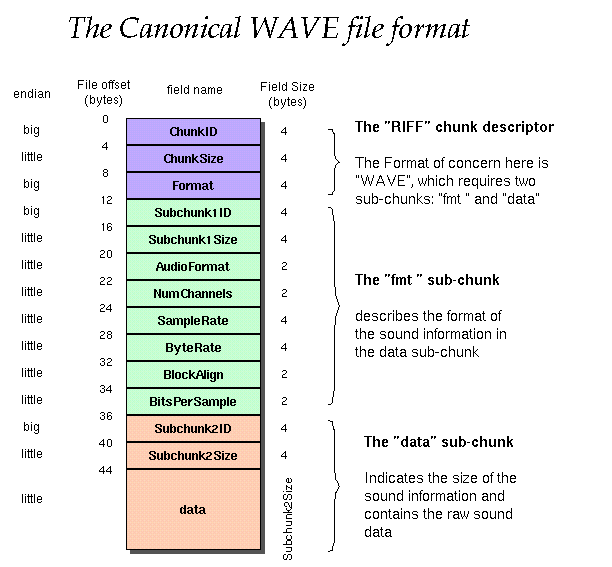
\includegraphics[width=8cm]{wav-sound-format.png}
\centering
\caption{Wave file format}
\end{figure}
\

\addcontentsline{toc}{subsection}{II.4.2. Python}
\subsection*{II.4.2. Python}

\

\verb|Python| is an interpreted high-level programming language for general-purpose programming. \verb|Python| provides constructs that enable clear programming on both small and large scales. It features a dynamic type system and automatic memory management. It supports multiple programming paradigms, including object-oriented, imperative, functional and procedural, and has a large and comprehensive standard library.
\\

There are available interpreters for many operating systems. \verb|CPython|, the reference implementation of \verb|Python|, is open source software and has a community-based development model. Because of the many resources and documentation for working with data. We used the following libraries in creating models (CNN and AdaBoost).
\\

\addcontentsline{toc}{subsubsection}{II.4.2.a. Sklearn}
\subsubsection*{II.4.2.a. Sklearn}

\

\verb|Scikit-learn| is a module Machine Learning in \verb|Python|. It provides diverse and efficient tools for data mining and data analysis that are accessible and has reusable in various contexts. It is built on \verb|NumPy|, \verb|SciPy|, and \verb|matplotlib|. Another bonus is that it is open source.
\\

\addcontentsline{toc}{subsubsection}{II.4.2.b. Keras}
\subsubsection*{II.4.2.b. Keras}

\

\verb|Keras| is a high-level neural networks API, written in \verb|Python| and capable of running on top of \verb|TensorFlow|, \verb|CNTK|, or \verb|Theano|. It was developed with a focus on enabling fast experimentation. Being able to go from idea to result with the least possible delay is key to doing good research. The guiding principles are: user friendliness, modularity, easy extensibility and work with \verb|Python|.
\\

We use \verb|TensorFlow| as back end for \verb|Keras| models. \verb|TensorFlow| is an interface for expressing machine learning algorithms, and an implementation for executing such algorithms. A computation expressed using \verb|TensorFlow| can be executed with little or no change on a wide variety of heterogeneous systems and can be used computational devices such as GPU cards. 
\\

\addcontentsline{toc}{subsection}{II.4.3. CUDA}
\subsection*{II.4.3. CUDA}

\

\verb|CUDA| (Compute Unified Device Architecture) is a parallel computing platform and programming model developed by \verb|NVIDIA| for general computing on graphical processing units (GPUs). It allows to use a \verb|CUDA|-enabled graphics processing unit (GPU) for general purpose processing.
\\

A big improvement in the results we obtain is using powerful and efficient parallel computing provided by GPU computing. GPUs are used to train deep neural networks using larger training sets, in an order of magnitude less time. We used GPU parallel computing power to speed up the training of the CNN.
\\

\newpage

\addcontentsline{toc}{chapter}{III. Results}
\chapter*{III. Results}

\

The experimental results on the two datasets can be compared with the three best methods in the Classifying Heart Sounds PASCAL Challenge. The evaluation of our models is performed on samples from the same datasets using the same evaluation criteria.
\\

In order to evaluate our method, we computed the total accuracy and we will present the confusion matrix for the categorical classifier. For the multi-task learning methods we will present the accuracy for discrimination extrastole, murmur and normal heartbeats, one from the others. We will show our accuracy and the results for the feature selection part.
\\

The data set we have for training has 451 recordings. After the processing steps we obtained 17901 segments of records, in the normal, extrastole and murmur classes. Out of these we use 15991 for training and the others for validation. These recordings have the following partition $[12549, 3648, 1527]$ in the normal, murmur and extrastole classes.
\\

The evaluation dataset consists of 30 recordings, segmented in $[102, 111, 104]$ segments of records in the normal, murmur and extrastole classes.
\\

\addcontentsline{toc}{section}{III.1. Feature selection}
\section*{III.1. Feature selection}

\

After the feature extraction phase we wanted to rank these features on their importance in classification. For this task we ran 3 classifiers (a Decision Tree, Random Forest and AdaBoost) and the results are presented in the following table.
\\

\begin{longtable}[!h]{ | m{0.6cm} | m{3.3cm} || m{2.3cm} | m{2.3cm} | m{2.3cm} | } 
\hline
No. & Feature & Decision tree importance & Random Forest importance & AdaBoost importance \\ 
\hline\hline
1 & Peak Frequency & 0.06358505 & 0.10835463 & 0.1 \\ 
\hline
2 & Peak Frequency Standard Deviation & 0.05584003 & 0.08143857 & 0.02 \\ 
\hline
3 & Peak Amplitude & 0.07775618 & 0.08109412 & 0.04 \\ 
\hline
4 & Peak Amplitude Standard Deviation & 0.05335595 & 0.07786953 & 0.12 \\ 
\hline
5 & Minimum Peak Distance & 0.22781165 & 0.12076171 & 0.28 \\ 
\hline
6 & Maximum Peak Distance & 0.0940705 & 0.10498685 & 0.18 \\ 
\hline
7 & Minimum Peak Amplitude & 0.03635814 & 0.07228694 & 0.02 \\ 
\hline
8 & Maximum Peak Amplitude & 0.03169072 & 0.07434332 & 0.04 \\ 
\hline
9 & Mean Amplitude & 0.15517295 & 0.11145975 & 0.02 \\ 
\hline
10 & Standard Deviation Amplitude & 0.18334003 & 0.15667982 & 0.14 \\ 
\hline
11 & Number of Peaks & 0.02251938 & 0.01072477 & 0.04 \\ 
\hline

\caption{Feature importance for 3 classifiers}
\end{longtable}


According to these results, the features that have the greatest impact in classifying the extrastole form the other heartbeats are: Minimum Peak Distance, Standard Deviation Amplitude, Mean Amplitude and Maximum Peak Distance.
\\

We will see the impact of these results in the accuracy of the AdaBoost model in the following section.
\\

\addcontentsline{toc}{section}{III.2. Classification results}
\section*{III.2. Classification results}

\

The results we obtained on the test data set is presented according the models we created: the multi-class CNN, the two CNN for normal and murmur datasets, and the AdaBoost Classifier. We present in this section the accuracy and the confusion matrix, beside other metrics. To better evaluate our models, we will take the result presented in section I.2 and compare them with the ones we obtained.
\\

The dataset is imbalanced so the model evaluation part was dificult. The test dataset has almost equals parts ot the 3 recording types. 
\newpage

\addcontentsline{toc}{subsection}{III.2.1. Multi-class CNN}
\subsection*{III.2.1. Multi-class CNN}

\

The accuracy representing how often the classifier gave the right answer, overall. The training accuracy resulted in the first epoch was 0.7615, followed by 0.9802. In order to avoid overfiting we used another dataset for validation. The validation dataset is not used for training, just for parameter optimisaton.
\\

The value of the loss function and the accuracy on the test dataset are the following:
\\

Test loss: 2.7176815245858754
\

Test accuracy: 65.74923552868927
\\

For a better understanding we present here the confusion matrix for the 3 class CNN we built. The recordings from the Normal class were in 87,6\% of cases classified correctly, the Murmur recordings we 80,7\%. The Extrastole category has about 30\% accuracy, most of the cases being confused with Normal heartbeats. A cause for this can be the fact that a extra sistole can apear between sounds, but are not periodical.
\\

[[92 20 71]
\

 [ 9 92  6]
 \
 
 [ 4  2 31]]
\\

\addcontentsline{toc}{subsection}{III.2.2. Normal heartbeats identification}
\subsection*{III.2.2. Normal heartbeats identification}

\

We created a CNN that selects the normal heartbeats from the others. The training accuracy resulted was 97,74\%. The value of the loss function and the accuracy on the test dataset are the following:
\\

Test loss: 2.9659911798774647
\

Test accuracy: 55.65749240942323
\\

The resulted confusion matrix can show us that the accuracy for the normal heatbeats classified as normal increased compared to the multi-class CNN, but the other sounds have a small accuracy.
\\

[[ 93 133]
\

 [ 12  89]]
\\

In the Classifying Heart Sounds PASCAL Challenge the results on the two datasets are: 46\% and 77\%, while we obtained a 55\% on the combined datasets.

\addcontentsline{toc}{subsection}{III.2.3. Murmur heartbeats identification}
\subsection*{III.2.3. Murmur heartbeats identification}

\

For identifing murmur heartbeats from the other types, we trained a CNN. The training accuracy resulted was 98,96\%. The value of the loss function and the accuracy on the test dataset are the following:
\\

Test loss: 1.2620686471279972
\

Test accuracy: 79.81651379792332
\\

The resulted confusion matrix can show us that the accuracy for the murmur heatbeats classified as normal decreased compared to the multi-class CNN, but the other sounds have a good result.
\\

[[ 62  14]
\

 [ 52 199]]
\\

In the Classifying Heart Sounds PASCAL Challenge the results on the two datasets are: 67\% and 37\%, while we obtained a 79\% on the combined datasets.
\\

\addcontentsline{toc}{subsection}{III.2.4. Extrastole heartbeats identification}
\subsection*{III.2.4. Extrastole heartbeats identification}

\

For the extrastole identification, we used an AdaBoost classiffier that uses as training data the features explained in the previous chapter. The test accuracy we obtained is:
\\

Test accuracy: 0.7003154574132492
\\

The resulted confusion matrix can show us that the accuracy for the extrastole heatbeats classified correct, decreased compared to the multi-class CNN, but the other sounds have a good result.
\\

[[ 19  10]
\

 [ 85 203]]
\\

In the Classifying Heart Sounds PASCAL Challenge the results on the two datasets are: 27\% and 67\%, while we obtained a 70\% on the combined datasets.
\newpage

\addcontentsline{toc}{section}{III.3. Contributions}
\section*{III.3. Contributions}

\

Some attempts to segment phonocardiograms (PCG) into heartbeats can be found in the literature. The characteristics of the PCG signal and other features such as heart sounds S1 and S2 location can be measured more accurately by digital signal processing techniques. We normalized the data using the $L^2$ norm and used a sliding window technique for which we used a peak detection algorithm. 
\\

In this thesis we extracted 11 features from time domain, frequency domain and statistical features that have potential to discriminate among the extrastole and other(normal and murmur) signals. Then we create models that we used in classification (CNN) and for the multi-task learning (CNN and AdaBoost). We compared the results with the ones presented in the Classifying Heart Sounds PASCAL Challenge and we present all the results in the corresponding chapter.

\newpage

\addcontentsline{toc}{chapter}{IV. Conclusion}
\chapter*{IV. Conclusion}

\

In this paper, we present a methodology for the Classifying Heart Sounds PASCAL Challenge. We propose an algorithm for S1 and S2 heart sound identification. We normalized the data using the $L^2$ norm and used a sliding window technique for which we used a peak detection algorithm. The models we used in classification are CNN and Adaboost. After the segmentation, we used two methods to train and classify the computed features into Normal, Murmur or Extrasystole (Extrasound).
\\

We think this is a good basis for further analysis of the heart sound signals. In future, the proposed method can also be implemented in latest mobile phones and can be used for early detection of some common heart diseases. This method would be extremely useful for the developing countries and for rural health management.
\\

The characteristics of the PCG signal and other features can be measured more accurately by digital signal processing techniques. We think we can improve our method by improving the correct identification of S1 and S2 in the segmentation and by finding new features that take advantage of this identification. As future improvement the FFT (Fast Fourier Transform) can provide a better understanding of the frequency contents of the heart sounds. An alternative way to analyse the non-stationary signals is the wavelet transform (WT). Despite its medical significance, developing signal processing techniques with great impact can be an application for machine learning.

%\nocite{*}
\addcontentsline{toc}{chapter}{Bibliography}

\bibliographystyle{unsrt}
\begin{thebibliography}{1}
\bibitem[1]{1} Global Health Estimates 2016: Deaths by Cause, Age, Sex, by Country and by Region, 2000-2016. Geneva, World Health Organization; 2018.

\bibitem[2]{2} The PASCAL Classifying Heart Sounds Challenge 2011, Bentley P. and Nordehn G. and Coimbra M. and Mannor S. Available: http://www.peterjbentley.com/heartchallenge/index.html

\bibitem[3]{3} Tison GH, Sanchez JM, Ballinger B, et al. Passive Detection of Atrial Fibrillation Using a Commercially Available Smartwatch. JAMA Cardiol. 2018;3(5):409–416. doi:10.1001/jamacardio.2018.0136

\bibitem[4]{4} Lumen Learning. Biology for Majors II https://courses.lumenlearning.com/wm-biology2/chapter/the-cardiac-cycle/

\bibitem[5]{5} http://soundfile.sapp.org/doc/WaveFormat/

\bibitem[6]{6} Gersh, Bernard J (2000). Mayo Clinic Heart Book. New York: William Morrow. ISBN 0-688-17642-9.

\bibitem[7]{7} Singh, Mandeep, Cheema, Amandeep. (2013). Heart Sounds Classification using Feature Extraction of Phonocardiography Signal. International Journal of Computer Applications. 77. 13-17. 10.5120/13381-1001. 

\bibitem[8]{8} M Debbal, S, bereksi reguig, Fethi. (2008). Frequency analysis of the heartbeat sounds. IJBSCHS. 13. 85-90. 

\bibitem[9]{9} Tamer Ölmez, Zümray Dokur, Classification of heart sounds using an artificial neural network, Pattern Recognition Letters, Volume 24, Issues 1–3, 2003, https://doi.org/10.1016/S0167-8655(02)00281-7.

\bibitem[10]{10} https://en.wikipedia.org/wiki/Heart\_murmur

\bibitem[11]{11} https://en.wikipedia.org/wiki/Heart\_arrhythmia
 
\bibitem[12]{12} Pete Chapman (NCR), Julian Clinton (SPSS), Randy Kerber (NCR), Thomas Khabaza (SPSS), Thomas Reinartz (DaimlerChrysler), Colin Shearer (SPSS) and Rüdiger Wirth (DaimlerChrysler) CRISP-DM 1.0 2000
 
\bibitem[13]{13} https://www.lifewire.com/wav-wave-files-2622395
 
\bibitem[14]{14} Philip de Chazal, M. O'Dwyer and R. B. Reilly, "Automatic classification of heartbeats using ECG morphology and heartbeat interval features," in IEEE Transactions on Biomedical Engineering, vol. 51, no. 7, pp. 1196-1206, July 2004. doi: 10.1109/TBME.2004.827359

\bibitem[15]{15} Weisstein, Eric W. L2-Norm. From MathWorld--A Wolfram Web Resource. http://mathworld.wolfram.com/L2-Norm.html

\bibitem[16]{16} Weisstein, Eric W. Vector Norm. From MathWorld--A Wolfram Web Resource. http://mathworld.wolfram.com/VectorNorm.html

\bibitem[17]{17} Scholkmann, Felix and Boss, Jens and Wolf, Martin An Efficient Algorithm for Automatic Peak Detection in Noisy Periodic and Quasi-Periodic Signals 2012 https://doi.org/10.3390/a5040588

\bibitem[18]{18} Krizhevsky, Alex, Sutskever, Ilya, E. Hinton, Geoffrey. (2012). ImageNet Classification with Deep Convolutional Neural Networks. Neural Information Processing Systems. 25. 10.1145/3065386. 

\bibitem[19]{19} https://www.techopedia.com/definition/869/sliding-window

\bibitem[20]{20} Guy Amit, Noam Gavriely, Nathan Intrator, Cluster analysis and classification of heart sounds, Biomedical Signal Processing and Control,2009, https://doi.org/10.1016/j.bspc.2008.07.003.

\bibitem[21]{21} Wenjie Zhang, Jiqing Han, Shiwen Deng, Heart sound classification based on scaled spectrogram and partial least squares regression, Biomedical Signal Processing and Control, 2017, https://doi.org/10.1016/j.bspc.2016.10.004.

\bibitem[22]{22} Randhawa, Simarjot, Singh, Mandeep. (2015). Classification of Heart Sound Signals Using Multi-modal Features. Procedia Computer Science. 58. 165-171. 10.1016/j.procs.2015.08.045. 

\bibitem[23]{23} Sebastian Ruder, An Overview of Multi-Task Learning in Deep Neural Networks, 2017

\bibitem[24]{24} Gomes, Elsa Ferreira and Emanuel Pereira. “Classifying heart sounds using peak location for segmentation and feature construction.” (2012).

\bibitem[25]{25} Deng, Yiqi. “A Robust Heart Sound Segmentation and Classification Algorithm using Wavelet Decomposition and Spectrogram.” (2012).

\bibitem[26]{26} H. Ryu, J. Park and H. Shin, "Classification of heart sound recordings using convolution neural network," 2016 Computing in Cardiology Conference (CinC), Vancouver, BC, 2016

\bibitem[27]{27} https://kaggle.com/kinguistics/heartbeat-sounds/kernels

\bibitem[28]{28} Ruihu Wang, AdaBoost for Feature Selection, Classification and Its Relation with SVM, A Review, Physics Procedia, Volume 25, 2012

\end{thebibliography}

%% F6 F11 F6 F6 Quick Build

\end{document}